\documentclass[12pt]{article}
\usepackage{fullpage}
\usepackage{times}
\usepackage[normalem]{ulem}
\usepackage{fancyhdr,graphicx,amsmath,amssymb, mathtools, scrextend, titlesec, enumitem}
\usepackage{graphicx}
\usepackage[cache=false]{minted}
\usepackage{wrapfig}
\usepackage[section]{placeins}


\title{C++ Memory Management}
\author{Alvin Grissom II}
\begin{document}
\maketitle
\section{Memory Organization}

It is important to understand the logical structure of memory in C++.
We use the term \textit{logical structure}, because this does not
reflect the physical structure of RAM, only how it is organized in
software.  We have the \textbf{free store/heap}, \textbf{stack}, and
areas for \textbf{const} data and \textbf{global} data.  The heap and
the stack can grow as needed (Figure 1)\footnote{Image from
  Wikipedia.}.  The stack starts with higher memory addresses and
grows downward; the heap starts with lower memory addresses and grows
upward.
\begin{wrapfigure}{r}{0.3\textwidth}
\centering 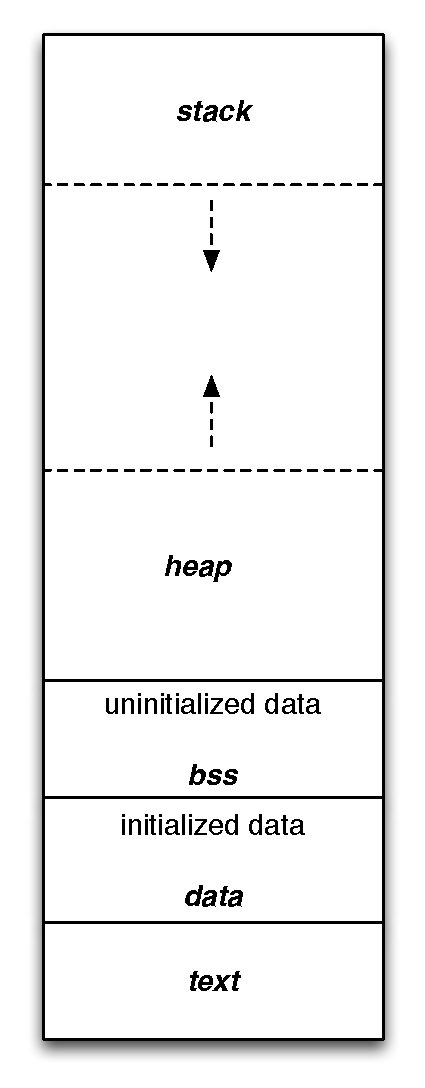
\includegraphics[scale=0.5]{figures/memory_layout.pdf}
\caption{Layout of C++ memory.  The lower memory addresses contain the
  global/static data, while the highest ones contain the stack.  The
  stack grows downward and the heap grows upward, as needed.}
\end{wrapfigure}

\textbf{The Stack}

The stack stores all function calls and variables local to them.
Recall that a stack is a LIFO data structure: the last item pushed is
the first popped. When a function call is on the stack, so are all of
its local variables.  Local variables are \textit{automatic
  variables}, because they are automatically destroyed when they go
out of scope.  These variables are all taken off the stack when the
function returns\footnote{This does not apply to memory allocated with
  \texttt{new}}.

\textbf{The Free Store}

The free store contains memory that is \textbf{dynamically allocated}
as needed.  This is usually implemented as a \textbf{heap} data
structure, and is therefore sometimes referred to as simply the heap,
as in Java.  Whenever the \texttt{new} keyword is used, dynamic
allocation takes place.  The \texttt{new} and \texttt{new[]} keywords
reserve just enough memory on the free store to store whatever kind of
data is appropriate for the type.  For every usage of \texttt{new},
there should be a corresponding \texttt{delete}, and for every usage
of \texttt{new[]}, there should be a corresponding \texttt{delete[]}.
A \textbf{pointer} is a variable that points to a memory address of a
given type. We must manage memory, not variables.  Variables only
serve as a way of gaining access to memory.
 
\textbf{The Global Namespace}

Global and static variables are stored in lower memory addresses
(Figure 1). The \textbf{bss} stores uninitialized data, and the
\textit{data} segment stores global and static variables initialized
in the program.  These are both allocated at \textit{compile time},
whereas the free store and stack are dynamically allocated at
\textit{runtime}.

\section{Memory Management}

A \textbf{pointer} is a variable that points to a memory
address. Pointer variables are allocated just as non-pointer
variables.  If they are defined inside of a function, they are
allocated on the stack and destroyed when the function completes; if
they are defined globally or statically, they are allocated in the
global namespace.  What the pointer \textit{points to}, however,
depends on how the data is allocated.

\begin{minted}[linenos, mathescape, obeytabs=false, frame=lines]{cpp}
int x; //stored in bss
int y = 5; //stored in data
int main(int argc, char** argv) {
    int y = 5; //stored on stack
    int * z = &y; //store on stack; value is memory address of y
    int a = *z; //stored on stack; value is 5
    return 0;
}
\end{minted}
\label{code:pointers1}
In the above example, you can determine in which memory area each
variable is stored based (1) on where it is defined in the code and
(2) whether or not it was initialized.  Since \texttt{main()} is a
function, all of its \textit{variables}, including pointer variables,
are stored on the stack.  Where global variables are stored depends on
whether or not they are initialized.  Somewhat confusingly, the
\texttt{*} operator serves two purposes: it is used to \textit{define
  a pointer} (line 5), and it is used to \textbf{dereference} pointers
(line 6). Dereferencing retrieves the value stored in the memory to
which the pointer points. When used as a dereferencer, \texttt{*} may
be read as ``the value store at'', and \texttt{\&} as ``address of''.
\subsection{Allocating Memory on the Free Store}
\begin{minted}[linenos, mathescape, obeytabs=false, frame=lines]{cpp}
int main(int argc, char** argv) {
    int y = 5; //stored on stack
    int * z = new int; //z stored on stack; value stored on heap
    int * arr = new int[10]; 
    //arr stored on stack; 10 int slots reserved on free store
    delete z;
    delete[] arr;
}
\end{minted}
\label{code:pointers2}

Often, you need the flexibility of the free store to
\textit{dynamically} allocate memory as needed. This is what
\texttt{new} and \texttt{new[]} allow you to do. They expand the free
store (heap) upward as needed at runtime, rather than reserve a fixed
(static) chunk of memory at compile time.

Above, we use the \texttt{new} operator to dynamically allocate memory
for a single \texttt{int} (line 3).  Every variable, including pointer
variables, that we create in a function is reserved on the stack, but
when we \textit{initialize} with \texttt{new}, we allocate memory for
its \texttt{data} on the free store.  On line 4, we reserve space for
10 \texttt{int} variables on the free store.  The variable
\texttt{arr} just points to a place in the free store where this
memory has been reserved.

\underline{\textbf{For every \texttt{new}, there should be a
    corresponding \texttt{delete}.}}  Calling \texttt{delete} frees up
the memory for later use.  For arrays, we need \texttt{delete[]},
because we need to clear out the entire array.  If we fail to
\texttt{delete} the memory we've allocated, we have a \textbf{memory
  leak}.

We are not freeing variables, but the memory to which they point.  If
we forget to free the memory we've reserved, the memory will be
\textbf{orphaned} and unrecoverable.  At times, you will need to use
temporary variables to allow you to appropriately delete memory when
you reassign dynamically allocated pointer variables.
\section{Pass by Reference}

C++ allows passing by reference.  This sometimes is an alternative to
using pointers.
\begin{minted}[linenos, mathescape, obeytabs=false, frame=lines]{cpp}
int main() {int a = 1; int b = 2; 
pointer_noswap(&a,&b); pointer_swap(&a, &b); reference_swap(a, b}
void pointer_noswap(int * x, int * y) { //wrong
    int * temp = x; //temp points to same address as x
    x = y; //x points address of y
    y = temp; //y points to old address of x
}
void pointer_swap(int * x,  int * y) {
    int temp = *x; //temp becomes value pointed to by x
    *x = *y; // value pointed to by x becomes value pointed to by y
    *y = temp; //value pointed to by y becomes old value of x
}
void reference_swap(int &x, int &y) {
   int temp = x; //set temp to value of a
   x = y;   //set x to value of b;
   y = temp   //set y to value of a
}
void noswap(int x, int y) { //copies values 1, 2 to x and y
    //Passes by value.  There is no way to make this work.
    int temp = x;  x = y;  y = temp;
}
\end{minted}
\label{code:point_ref}
The \texttt{swap()} function should swap the \textit{original} values
passed to it, not the copied values.

\textbf{Case 1} We pass in the address of a and b.  In this case, the
values \texttt{x} and \texttt{y} are the memory addresses of
\texttt{a} and \texttt{b}, respectively. The variable \texttt{temp}
stores the address of \texttt{x}, and \texttt{x} is set to the address
of \texttt{y}. Then the value to which \texttt{y} points is the memory
address of temp. This line won't even compile without a cast, because
the \texttt{int*} and \texttt{int} are different types. The logic is
also wrong.

\textbf{Case 2} Again the memory addresses of \texttt{a} and
\texttt{b} are passed in by value.  The values of \texttt{x} and
\texttt{y} are swapped explicitly with \textit{dereferencing}, but the
memory addresses of \texttt{a} and \texttt{b} are not swapped.

\textbf{Case 3} We pass in \texttt{a} and \texttt{b} \underline{by
  reference}.  So, \texttt{x} and \texttt{y} are actually the same as
\texttt{a} and \texttt{b}! The variable \texttt{temp} is set to the
value pointed to by \texttt{x}, and then the values of \texttt{x} and
\texttt{y} are swapped.

\textbf{Case 4} We pass in the values of \texttt{a} and \texttt{b}
\textit{by value}.  This means \texttt{x} and \texttt{y} are set to 1
and 2, but they are not the same variables as \texttt{a} and
\texttt{b}.  Even though we swap \texttt{x} and \texttt{y}, we don't
swap \texttt{a} and \texttt{b}.

\section{Class Memory Management}

\textbf{Destructors} are the foil of constructors.  A constructor is
called when an object is constructed; a destructor is called when an
object is destroyed.  The primary purpose of the destructor is to free
any class-level memory has not been freed.  The destructor, like the
constructor, has no return type and must have the same name as the
class.  The difference is the the destructor's name beings with a
\texttt{\~}.

\begin{minted}[linenos, mathescape, obeytabs=false, frame=lines]{cpp}
class MyClass {
  public:
    MyClass(); //constructor declaration  
    ~MyClass(); //destructor declaration
  private:
    int * arr //variable stored inside object
};
MyClass::MyClass() {
    array = new arr[10]; //memory allocated on free sore
}
MyClass::~MyClass() {
    delete[] array; //memory freed at object's destruction
}
\end{minted}
\label{code:destructor}

We allocate memory for an array (l. 10).  Thus, when the class is
destroyed, we want to be sure that everything is cleaned up, i.e., all
free store-allocated memory has been freed.  If we did not have the
\texttt{delete[]} call, every instance of my class would leak the
memory for 10 integers.
\subsection{Copy Constructors}
There are two ways of ``copying'' an object: a \textbf{deep copy} and
a \textbf{shallow copy}.  A shallow copy creates a duplicate of the
original object. If it has any pointers, the object's copies of them
will still point to the same locations as the pointers in the
original; so, modifying data in the original object modify it in the
copy. A deep copy creates \textit{copies} of the data pointed to in
the original object, so modifying the copy won't affect the original
and vice versa. E.g., suppose the original object has an
array. Instead of pointing to the original array in the clone, a deep
copy would create a new array elsewhere in memory, point to it
instead, and copy all of the data from the original to the new array.
By default, C++ will do a shallow copy whenever the assignment
operator is used on an object. This is in contrast to Java, where
every object is a pointer (reference).
\begin{minted}[linenos, mathescape, obeytabs=false, frame=lines]{cpp}

int main() {
    Cat a = Cat(); //no pointer used
    Cat b = a;  //copy constructor called, deep copy a to b.
    Cat * d = new Cat(); // d is a pointer;
    Cat * e = d; //copy constructor NOT called. d, e point to same Cat
    Cat * f = new Cat(d); //copy constructor called, deep copy
}
class Cat {}
  public:
    Cat();
    int getNumToys();
    std::string * getToys();
    Cat(const Cat &c);
   private:
     std::string * toys; 
     int numToys;
};
int Cat::getnumToys() { return numToys; }
std::string * getToys() { return toys; }
Cat::Cat() {
    numToys = 0;
    toys = new std::string[5];
}
Cat::Cat(const Cat &c) {
    this->numToys = c.getNumToys();
    this->toys = new std::string[c.getNumToys()];
    for(int i = 0; i < c.getNumToys(); i++) {
        this->toys[i] = c.getToys()[i]; 
    }
}
Cat::~Cat() { delete[] toys; }
\end{minted}
The copy behavior of an object is \textit{user-defined.}\footnote{The
  C++ compiler creates default copy constructors that do a shallow
  copy.}  To define how to copy an object, we need a \textbf{copy
  constructor}.  A copy constructor is a constructor that takes as an
argument an object of the same type as the object being constructed.



In the code above, the \texttt{Cat} class has a dynamically allocated
array.  Our copy constructor (line 156) takes a \texttt{const}
(immutable) reference to the original \texttt{Cat} object and
duplicates each element in its array.  This performs a deep copy, so
modifying the array created by the copy constructor won't change
anything in the original, and vice versa.  The \texttt{const} modifier
ensures that we won't accidentally modify the original object.

We can see on lines 5-8 that the copy constructor is \textit{not}
called when reassigning the \textit{pointers} that point to objects.
In this case, the semantics are similar to Java's.  However, we can
make an explicit call to the copy constructor (line 8) to create a
pointer to a copy of the original object.

\subsection{Why use pointers to objects?}

In Java, all object variables are pointers (or ``references,'' in
Java's language), so when a function has an object as a function
parameter, instead of passing the corresponding object and all of its
information, only the memory address is passed.  In C++, however,
passing in objects performs a shallow copy of the object into the
method's scope.  This is computationally expensive and takes up
potentially a large amount of RAM.  One way of mitigating this is to
pass in a pointer (or pass by reference).  Copying a single memory
address will always be more efficient than copying all of an object's
internal variables.  Unless there is a good reason to do otherwise, it
is always preferable to pass a pointer or pass by reference, rather
than pass in an object by value.
\section{new is the new malloc}
The C programming language, which preceded C++, does not have the
\texttt{new} keyword.  Instead, it has \texttt{malloc},
\texttt{calloc}, and related functions.  The \texttt{malloc} function
is how one reserves memory in the free store in C.  It requires that
the programmer specify how much memory is to be reserved and returns
the starting address for the reservation.

\texttt{void* malloc (size\_t size )}.  

The \texttt{size\_t} type is a numerical value for representing the
size of types in bytes.  It returns a \texttt{void*}, which is a
pointer to any type. \texttt{malloc} returns a pointer to the first
memory address in the chunk that it reserves.

\texttt{int * array = (int *) malloc( 10 * sizeof(int) );}

This reserves enough space for ten \texttt{int}s and returns a pointer
to the the first one.  It casts this pointer to an \texttt{int *}.  In
C, when we are finished with this reserved memory, we call
\texttt{free(array)} to release it.  In C++, instead of
\texttt{malloc()} and \texttt{free()}, we use \texttt{new} and
\texttt{delete} or \texttt{new[]} and \texttt{delete[]}, and the
amount of RAM to be reserved is handled by \texttt{new}.

\end{document}
